\section{Theorie}
\label{sec:Theorie}


% 2x2 Plot
% \begin{figure*}
%     \centering
%     \begin{subfigure}[b]{0.475\textwidth}
%         \centering
%         \includegraphics[width=\textwidth]{Abbildungen/Schaltung1.pdf}
%         \caption[]%
%         {{\small Schaltung 1.}}
%         \label{fig:Schaltung1}
%     \end{subfigure}
%     \hfill
%     \begin{subfigure}[b]{0.475\textwidth}
%         \centering
%         \includegraphics[width=\textwidth]{Abbildungen/Schaltung2.pdf}
%         \caption[]%
%         {{\small Schaltung 2.}}
%         \label{fig:Schaltung2}
%     \end{subfigure}
%     \vskip\baselineskip
%     \begin{subfigure}[b]{0.475\textwidth}
%         \centering
%         \includegraphics[width=\textwidth]{Abbildungen/Schaltung4.pdf}    % Zahlen vertauscht ... -.-
%         \caption[]%
%         {{\small Schaltung 3.}}
%         \label{fig:Schaltung3}
%     \end{subfigure}
%     \quad
%     \begin{subfigure}[b]{0.475\textwidth}
%         \centering
%         \includegraphics[width=\textwidth]{Abbildungen/Schaltung3.pdf}
%         \caption[]%
%         {{\small Schaltung 4.}}
%         \label{fig:Schaltung4}
%     \end{subfigure}
%     \caption[]
%     {Ersatzschaltbilder der verschiedenen Teilaufgaben.}
%     \label{fig:Schaltungen}
% \end{figure*}

\subsection{Erzeugung der Röntgenstrahlung}

Für die Erzeugung von Röntgenstrahlung können verschiedene Methoden verwendet werden.
Im vorliegenden Versuchsaufbau wird die Strahlung mithilfe beschleunigter Elektronen erzeugt, welche an einem Glühdraht durch den glühelektrischen Effekt erzeugt werden.
Die Elektronen werden beschleunigt und auf eine Anode aus einem bestimmten Material geschossen, wodurch auf zwei verschiedene Arten Röntgenstrahlung entsteht.
Zunächst entsteht die sogenannte Bremsstrahlung, bei denen die kinetische Energie der Elektronen vollständig durch die Ablenkung bzw. Abbremsung in Röntgenstrahlung mit der minimalen Wellenlänge
\begin{equation}
  \lambda_{\text{min}} = \frac{h c}{e_0 U}
\end{equation}
umgewandelt wird.
Dementsprechend handelt es sich bei der Bremsstrahlung um ein kontinuirliches Spektrum, welches durch die Wahl der Beschleunigungsspannung begrenzt wird.\\
Des Weiteren entsteht die durch das Anodenmaterial bestimmte charakteristische Strahlung.
Diese entsteht, wenn das beschleunigte Elektron das Atom ionisiert.
Hierbei muss ein Elektron aus der äußeren Schale das gerade ionisierte Elektron ersetzen, so dass bei diesem Übergang Strahlung emittiert werden.
Aufgrund der diskreten Energieniveaus ergeben sich auch diskrete Frequenzen der Röntgenstrahlung, welche dem Wert
\begin{equation}
  h f = E_{\text{m}} - E_{\text{n}}
\end{equation}
entsprechen.
Die verwendete Notation ist es dabei, die entstehenden Linien im Röntgenspektrum beispielsweise mit $K_{\alpha}$ zu bezeichnen, wobei $K$ die Schale benennt, in der der Übergang endet, und der Index die Anzahl die Anzahl der gesprungenen Schalen.\footnote{Beispielsweise $\alpha \hat{=} 1$, $\beta \hat{=} 1$, usw.}
Die Bindungsenergien werden dabei im Allgemeinen durch die Formel
\begin{equation}
  E_n = - R_{\infty} z_{\text{eff}}^2 \frac{1}{n^2}
\end{equation}
für die Bindungsenergie eines Elektrons der n-ten Schale beschrieben.
Hierbei ist $R_{\infty}$ die Rydbergenergie und $z_{\text{eff}} = z - \sigma$ die effektive Kernladung mit der für das jeweilige Elektron im Atom charakteristische Abschirmkonstante $\sigma$.
Neben der Hauptquantenzahl $n$ besitzen die Elektronen noch weitere Quantenzahlen, resultierend aus dem Elektronenspin und dem Bahndrehimpuls, so dass eine weitere, feinere Aufspaltung der Linien möglich ist.
Die Energien dieser Feinstruktur lassen sich mithilfe der Sommerfeldschen Feinstrukturformel nach
\begin{equation}
  E_{\text{n}, \text{j}} = -R_{\infty} \Bigl(  \frac{z_{\text{eff},1}^2}{n^2} + \alpha^2  \frac{z_{\text{eff},2}^4}{n^3} \Bigl( \frac{1}{j+\frac{1}{2} - \frac{3}{4n} }  \Bigr)  \Bigr)
\end{equation}
berechnen, wobei $j$ der Gesamtdrehimpuls des Elektrons und $\alpha$ die Sommerfelsche Feinsturkturkonstante ist.

\subsection{Absorption von Röntgenstrahlung}
Bei dem Auftreffen von Röntgenstrahlung auf einen Absorber wird Röntgenstrahlung absorbiert, wobei hier ähnlich wie bei der Erzeugung von Röntgenstrahlung für das Material charakteristische diskrete Phänomene auftreten.
Im Allgemeinen nimmt die Fähigkeit zur Absorption, beschrieben durch den Absorptionskoeffizient, mit sinkender Wellenlänge der Röntgenstrahlung ab.
Bei diskreten Werten treten jedoch Sprünge auf, welche stattfinden, wenn die Energie der Röntgenstrahlung ausreicht, um die Bindungsenergie eines weiteren Elektrons im Absorbermaterial zu ionisieren.
Hierbei treten Absorptionskanten für die Wellenlängen
\begin{equation}
  \lambda_{\text{abs}} = \frac{h c}{E_{\text{n}} - E_{\infty}}
\end{equation}
auf.\\

Im vorliegenden Versuch kann die Abschirmkonstante $\sigma_{\text{L}}$ nach der Formel
\begin{equation}
  \sigma_L = Z - \Bigl( \frac{4}{\alpha} \sqrt{ \frac{\increment E_{\text{L}} }{R_{\infty}}} - \frac{5 \increment E_{\text{L}} }{R_{\infty}}     \Bigr)^{0.5} \Bigl( 1 + \frac{19}{32} \alpha^2 \frac{\increment E_{\text{L}} }{R_{\infty}} \Bigr)^{0.5}
\end{equation}
bestimmt werden, wobei $Z$ die Ordnungszahl und $\increment E_{\text{L}} = E_{\text{L, II}} - E_{\text{L, III}}$ die Energiedifferenz zwischen zwei $L$-Kanten ist.

\subsection{Analyse des Röntenspektrums über die Bragg-Reflexion}
Um das Röntgenspektrum hinsichtlich seiner Intensität in Abhängigkeit von der Wellenlänge untersuchen zu können, wird ein Kristall mit gegebener Gitterkonstanten $d$ verwendet.
Die in einem bestimmten Winkel $\theta$ auf den Kristall auftreffende Strahlung wird, wie in Abbildung \ref{abb:2} dargestellt, am Gitter gebeugt, so dass Interferenz entsteht.
\begin{figure}[H]
  \centering
  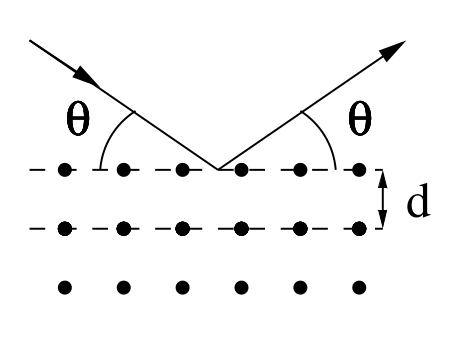
\includegraphics[height=5cm]{ressources/bragg.png}
  \caption{Schematische Darstellung der Bragg-Reflexion.\cite{skript}}
  \label{abb:2}
\end{figure}
Für den Glanzwinkel $\theta_{\text{glanz}}(\lambda)$ tritt konstruktive Interferenz auf, so dass die Strahlung hier verstärkt wird.
Die Wellenlänge zum zugehörigen Winkel lässt sich aus der Bragg-Bedingung zu
\begin{equation}
  \lambda = \frac{2 d \sin{\Theta}}{n}
\end{equation}
bestimmen, wobei $n$ die Ordnung des Maximums beschreibt.
